\textbf{Фазовая скорость}. 
В терминах фазовой скорости можно записать, что
\begin{equation*}
    u(x, t) = a\cos(kx-\omega t) = a \cos\left[k(x- \sub{v}{ф} t)\right],
\end{equation*}
то есть со скоростью $\sub{v}{ф}$ перемещается точка волны, фаза которой имеет фиксированной значение: $\varphi(x, t) = \omega  t - k x = \const$. В общем случае связь частоты и волнового числа определяется законом дисперсии $\omega = \omega(k) = \omega(\lambda)$. 



\begin{to_def}
    \textit{Фазовой скоростью} называют величину $\sub{v}{ф} = \omega/k = c/n$.
\end{to_def}


\begin{to_def}
    Зависимость фазовой скорости от длины волны -- \textit{дисперсия}.
\end{to_def}



\textbf{Групповая скорость}. Рассмотрим две волны со скоростями $\omega_1$ и $\omega_2$ с соответсвующими $k_1(\omega_1)$ и $k_2(\omega_2)$. Пусть волны задаются уравнениями
\begin{equation*}
    \left.\begin{aligned}
        u_1 &= a \sin (k_1 x - \omega_1 t) \\
        u_2 &= a \sin(k_2 x - \omega_2 t)
    \end{aligned}\right.
    \hspace{0.5cm} \Rightarrow \hspace{0.5cm}
    u(x, t) = u_1 + u_2 = 2 a \cos\left[
        \frac{k_2-k_1}{2}x - \frac{\omega_2-\omega_1}{2}t
    \right] \sin\left[
        \frac{k_2 + k_1}{2}x - \frac{\omega_2+\omega_1}{2}t
    \right].
\end{equation*}
Логично ожидать, что $k_2-k_1 \ll k_1$, тогда считая $k = \langle k_1,\,  k_2\rangle$,  $\omega = \langle \omega_1,\, \omega_2\rangle$ и $k_2 - k_1 = \Delta k$, $\omega_2-\omega_1 = \frac{d \omega}{d k} \Delta k$, перепишем выражение в виде
\begin{equation*}
    u(x, t) = 2 a \cos\left[
        \frac{\Delta k}{2} \left(
            x - \frac{d \omega}{d k} t
        \right)
    \right] \cdot \sin(kx - \omega t),
\end{equation*}
что очень сильно напоминает биения. Получается, что рассматривая эволюцию волны во времени корректно ввести \textit{групповую скорость} $\sub{v}{гр} = \d\omega/\d k$, -- при таком движении модуляция волны сохраняет фиксированное значение. Это обобщается и на некоторый диапазон $k_i$, тогда получим выражение вида
\begin{equation*}
    u(x, t) = \exp\left[i(kx-\omega t)\right] F(x- \sub{v}{гр}t).
\end{equation*}
Именно с функцией $F(x- \sub{v}{гр}t)$ связывают представление о цуге волн, или \textit{волновом пакете}. 


\textbf{Формула Рэлея}. Найдём связь фазовой и групповой скоростей: считая $\omega = k \sub{v}{ф}$ находим сотношение вида
\begin{equation*}
    \sub{v}{гр} = \sub{v}{ф} - \lambda \frac{d \sub{v}{ф}}{d \lambda}, 
\end{equation*} 
которое называют \textit{формулой Рэлея}. 

Свяжем групповую скорость волны с показателем преломления. Из формулы Рэлея:
\begin{equation*}
    \sub{v}{гр} = \sub{v}{ф} - \lambda \frac{d }{d \lambda} \left(\frac{c}{n}\right) = 
    \sub{v}{ф} \left(1 + \frac{\lambda}{n} \frac{d n}{d \lambda} \right) = 
    \frac{c}{n + \omega \ d n / \d \omega}
    .
\end{equation*}
Однако также верно, что $\lambda = \frac{2 \pi c}{n \omega}$, так что корректнее иметь производну. по частоте. 



\textbf{Нормальная и аномальная дисперсия}. Пусть $\sqrt{\varepsilon} = n + i \kappa$. Величина $n = \Re\sqrt{\varepsilon}$ -- \textit{показатель преломления}, и $\kappa = \Im \sqrt{ \varepsilon}$ -- \textit{показатель поглощения} (затухания). 


Представляя атомы осцилляторами с собственной частотой $\omega_0 = \sqrt{\beta/m}$ и коэффициентом затухания $\gamma = \eta/2m$ можно для концентрации атомов $N$ найти проницаемость
\begin{equation*}
    \varepsilon = 1 + \frac{\omega_p^2}{\omega_0^2 - \omega^2 - 2 i \gamma \omega}, \hspace{5 mm} 
    \omega_p^2 = 4 \pi N \frac{e^2}{m}. 
\end{equation*}
Вообще можно выделить нормальну ($n'_\omega > 0$) и аномальную ($n'_\omega < 0$) дисперсию, подробнее на рис. \ref{fig:abn}. 
\begin{figure}[h]
    \centering
    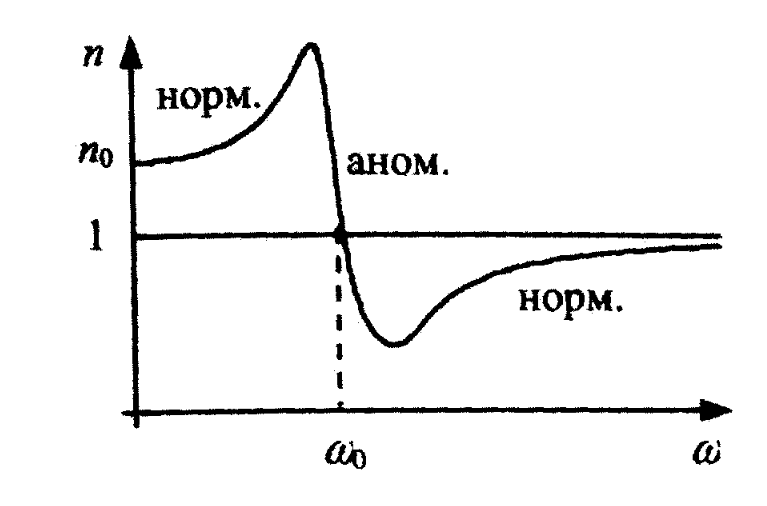
\includegraphics[width=0.3\textwidth]{figures/k10_1.png}
    \caption{Аномальная и нормальная дисперсия}
    \label{fig:abn}
\end{figure}
Для случая, когда $\varepsilon(\omega)$ не сильно отличается от $1$, можно получить следующие выражения
\begin{equation*}
    n = 1 + \frac{\omega_p^2}{2} \frac{\omega_0^2-\omega^2}{(\omega_0^2-\omega^2)^2 + 4 \gamma^2 \omega^2}, \hspace{5 mm} 
    \kappa = \frac{\gamma \omega_p^2 \omega}{(\omega_0^2-\omega^2)^2+4 \gamma^2 \omega^2}.
\end{equation*}


\textbf{Закон Бугера}. Чуть подробнее раскрывая показатель поглощения:
\begin{equation*}
    k = \frac{\omega}{c} \sqrt{\varepsilon} = \frac{\omega}{c} n + i \frac{\omega}{c}\kappa,
\end{equation*}
где вводится $\alpha = \frac{4\pi}{\lambda_0} \kappa$ и $\lambda_0 = \frac{2 \pi c}{\omega}$ -- длина волны излучения в вакууме на частоте $\omega$. Итого, для бегущей волны получается
\begin{equation*}
    E \sim e^{ik_r x} e^{- \alpha x/2},
    \hspace{0.5cm} \Rightarrow \hspace{0.5cm}
    I = I_0 e^{- \alpha x},
\end{equation*}
что и называют \textit{законом Бугера}. 





\textbf{Закон Лоренца-Лоренца}. Когда велика концентрация свободных электронов значимым становится поле электронов, действующее на остальные, что может быть сравнимо с действием внешнего поля. Так можем связать $\varepsilon$ и поляризуемость отдельных молекцл $\beta$ 
\begin{equation*}
    \varepsilon = \frac{1 + \frac{8\pi}{3} N \beta}{1 - \frac{4\pi}{3} N \beta},
    \hspace{0.5cm} \Rightarrow \hspace{0.5cm}   
    \frac{4 \pi}{3} N \beta = \frac{\varepsilon-1}{\varepsilon+1},
\end{equation*}
что называют \textit{формулой Лоренца-Лоренца}. 



